\label{sec:model}

In this section an example of a classical mathematical model for
offline optimization will be presented along with a model, which
allows for more dynamic systems. The objective function used in an
offline optimizer does not consider multiobjectivity but could be
replaced by a more refined performance measure.

The following notation is used:

\begin{table}[!ht]
\begin{center}
\begin{tabular}{ll}
\hline
$n \in \lbrace 1,...,N \rbrace$ & Intersection indexes \\
$p \in \lbrace 1,...,P_n \rbrace$ & Indexes of phases at intersection $n$ \\ 
$\Psi$ & A set of signal timing settings \\
$C_n$ & Cycle time for intersection $n$ \\
$\theta_n$ & Offset of intersection $n$ \\
$\phi_{np}$ & Phase $p$ green time for intersection $n$  \\
$I_{np}$ & Interstage (lost) time from the end of phase $p$ until the next  \\
\hline
$l \in \lbrace 1,...,L \rbrace$ & Link indexes \\
$q_l \in \textbf{q*}(\Psi)$ & User equilibrium link flows given signal timing parameters  \\
$t_l(\Psi,\textbf{q*}(\Psi))$ & Travel time on link $l$ considering signal timings and user response \\
\hline
\end{tabular}
\end{center}
\caption{Notation for the traffic signal and network model part}
\end{table}

\subsubsection*{A classical model}

The problem is formulated as the minimization of a MOE in terms of a
set of signal settings, $\Psi$, and a network of user equilibrium link
flows (see section \ref{sec:usereq}), $\textbf{q*}(\Psi)$, which is
dependent on the signal settings.

Teklu \cite{2} presents a model which is typical for offline optimizers, which is given here with slight modifications:

\begin{eqnarray}
\min & TT(\Psi, \textbf{q*}\left( \Psi\right)) = \displaystyle\sum_{l = 1}^{L} q_l \cdot t_l(\Psi,\textbf{q*}(\Psi))
\end{eqnarray}
\begin{eqnarray}
\label{eqn:cycletimeconstraints} subject\;to:\;C_{min,n} \leq C_n \leq C_{max,n} & \\
\label{eqn:offset} 0 \leq \theta_n \leq C_n-1 & \forall n \\
\label{eqn:greentimelimits} \phi_{min,np} \leq \phi_{np} \leq \phi_{max,np} & \forall n,p \\
\label{eqn:commoncycledef} C_n = \sum_{p=1}^{P_n} ( \phi_{np} + I_{np} ) & \forall n
\end{eqnarray}

In \cite{2} the chosen MOE is the travel time defined as the sum of flow
multiplied by travel time on each link and $\Psi = \lbrace
C,\theta,\phi \rbrace$. The user equilibrium flows are calculated
using a variational inequality, which is not reprinted here
considering the scope of the survey.

The sum of green- and lost time for all phases of an intersection must
equal the cycle time as seen in equation
(\ref{eqn:commoncycledef}). Equations (\ref{eqn:cycletimeconstraints})
and (\ref{eqn:greentimelimits}) are safeguards entered by traffic
engineers to avoid extreme plans such as the total suppresion of green
time for a minor road or very high cycle times (capacity), which would
otherwise be chosen under congestion. Equation (\ref{eqn:offset})
adjusts the offsets so as to create green waves but is only relevant
in the common cycle time model, which is a special case of the
presented model when $\forall n : C_n = C$. Offset is always
considered as a modulus of a \textit{common} cycle time and thus no
coordination can be made (in this model) if all intersections run on
their own clock.

In addition to this deficiency this model does not consider phase
sequences. Phases are simply enumerated and allocated green time - the
order is assumed given.

\subsubsection*{A dynamic model}
\label{sec:dynamicmodel}

In a general discrete time model time is indexed by $t \in H = \lbrace
t_{min},...,t_{max} \rbrace$ and thus $H$ indicates the horizon of the
optimization. \cite{36} containes an example of a general
continuous model, with has similarities to the presented model that
will be presented in this section. Each signal is designated a phase
for each time unit. Thus the concept of a cycle becomes virtual as
they are no longer mandatory for calculating eg. the length of phases
given the green splits.

Without a common cycle time - or individual cycle time, even - the
offset parameter also disappears. However they can be introduced
virtually, in terms of a virtual cycle, and can thus be manipulated to
excert the same behaviour.  The main problem is during initialization
when the system has just started. In this case it is possible to
synchronize intersections by delaying startup for those that would
otherwise have a positive offset. The same strategy can be used when
changing the (virtual) cycle time for the arterial. As discussed in
the previous chapter, the common cycle time and offsets requires a
periodicity, which is restrictive, and thus the inclusion of these
concepts into a dynamic model will not be discussed further.

Phase sequences and green splits are unified by the specification of the phase in a timeslot, $t$, referred to as $p_n(t)$. For each intersection there will be a fixed number of phases, $P_n$, which are free from right-of-way conflicts. For a simple cross intersection with left-side driven vehicles (see Figure \ref{fig:simple_intersection}) this number is 2: straight, left, and right turning flows in north and south directions for phase 1 and in east and west directions for phase 2.

\begin{figure}[!ht]
\begin{center}
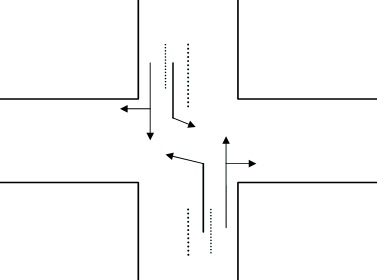
\includegraphics[scale=0.4]{simple_intersection.png} 
\end{center}
\caption{Simple 2-phase intersection}
\label{fig:simple_intersection}
\end{figure}

Thus a specific phase $p = p_n(t) \in \lbrace 1,...,P_n \rbrace$ is selected for each timeslot. With this definition the green splits are implicit in the phase sequence and we have $\Psi = \lbrace \textbf{p} \rbrace $.

In the following some constraints will be defined to show that the dynamic model is capable of satisfying constraints such as the ones for the classical model. Initially the set of consecutive timeslots allocated to phase $p$ for intersection $n$ is defined:

\begin{equation}
T_{pn} = \bigcup_{T = \lbrace t_1,...,t_2 \rbrace} \; st. \; p \not \in \lbrace p_n(\min T - 1), p_n(\max T + 1) \rbrace \wedge\forall t \in T: p_n(t) = p 
\end{equation}

Thus $T_{pn}$ is a set of sets and each containing a consecutive number of time units which bounds the extend of a particular phase.

Satisfaction of minimum and maximum green times is the most common
constraint, usually defined within a cycle. In the dynamic model this
constraint is formulated so that the minimum and maximum green times
must be respected over the entire horizon in the following equation:

\begin{equation}
\label{eqn:minmaxtimes}
\forall p,n : T_{min,pn} \leq |\underline{T_{pn}}| \wedge |\overline{T_{pn}}| \leq T_{max,pn} 
\end{equation}

The operators $\underline{T}$ and $\overline{T}$ are used to extract the smallest and largest sets (cardinality) from $T$.

That is, the length of all consecutive series of time slots in which
phase $p$ is run, must satisfy the selected minimum and maximum green
times. This constraint only demands that no phases are given too
little or too much time. It is also necessary to ensure that phases
are given green time in some minimum and maximum proportion to the
other phases of the intersection.

\begin{equation}
\label{eqn:proportions}
\forall p,n : R_{min,pn} \leq \frac{\sum |T_{pn}|}{|H|} \leq R_{max,pn}
\end{equation}

Where $|H|$ is the number of time steps in the signal timing plan so
far and $R_{min,pn}$ and $R_{max,pn}$ is the minimum and maximum
ratios of time over the optimization horizon, which is allowed for
phase $p$ at intersection $n$. It is clear that $\forall n :
\displaystyle\sum_{p=1}^{P_n}\frac{|T_{pn}|}{|H|} = 1$ due to the
definition of the phase specification function, $p_n(t)$, ie. in each
time slot a signal controlled intersection is assigned to a particular
phase.

Considering the north-south direction (phase 1) of figure
\ref{fig:simple_intersection} to lie along an arterial and the
east-west direction (phase 2) being a minor road the min and max
ratios could set like in Table \ref{tbl:minmaxratios}.

\begin{table}[!ht]
\begin{center}
\begin{tabular}{c|c|c}
$p$ & $R_{min,p}$ & $R_{max,p}$ \\ \hline
1 & $0.6$ & $0.8$ \\ 
2 & $0.2$ & $0.4$
\end{tabular}
\end{center}
\caption{Example of minimum and maximum green time ratios for a simple, 2-phase intersection}
\label{tbl:minmaxratios}
\end{table}

Together equations \ref{eqn:minmaxtimes} and \ref{eqn:proportions},
along with proper minimum and maximum values, ensure that green time
is distributed evenly over the optimization horizon since
\ref{eqn:proportions} ensures that the proportions are correct and
\ref{eqn:minmaxtimes} makes sure allocated green time is not bunched
together in some narrow part of the horizon.

These specifications result in a model which is relatively easy to
represent but may be difficult to fit into the standard mixed-integer
programming (MIP) scheme. An alternative is to use a metaheuristic
procedure, or the application of a set partitioning model (SPP), for
instance with column generation.
